\section{Введение}

Приложения, обрабатывающие большие объёмы данных, используют фраемворки, позволяющие производить вычисления с состоянием над ограниченными и неограниченными потоками данных, такие как, например, Apache Flink \cite{flink-org}.

Подобные фраемворки обычно запускаются на кластере машин, получают запросы на обработку данных от приложений, берут данные из источников, производят обработку в соответствии с запросом и формируют результат в виде записи в базе данных или в виде нового потока (см. рис. \ref{fig:flink-app}).

\begin{figure}[h]
    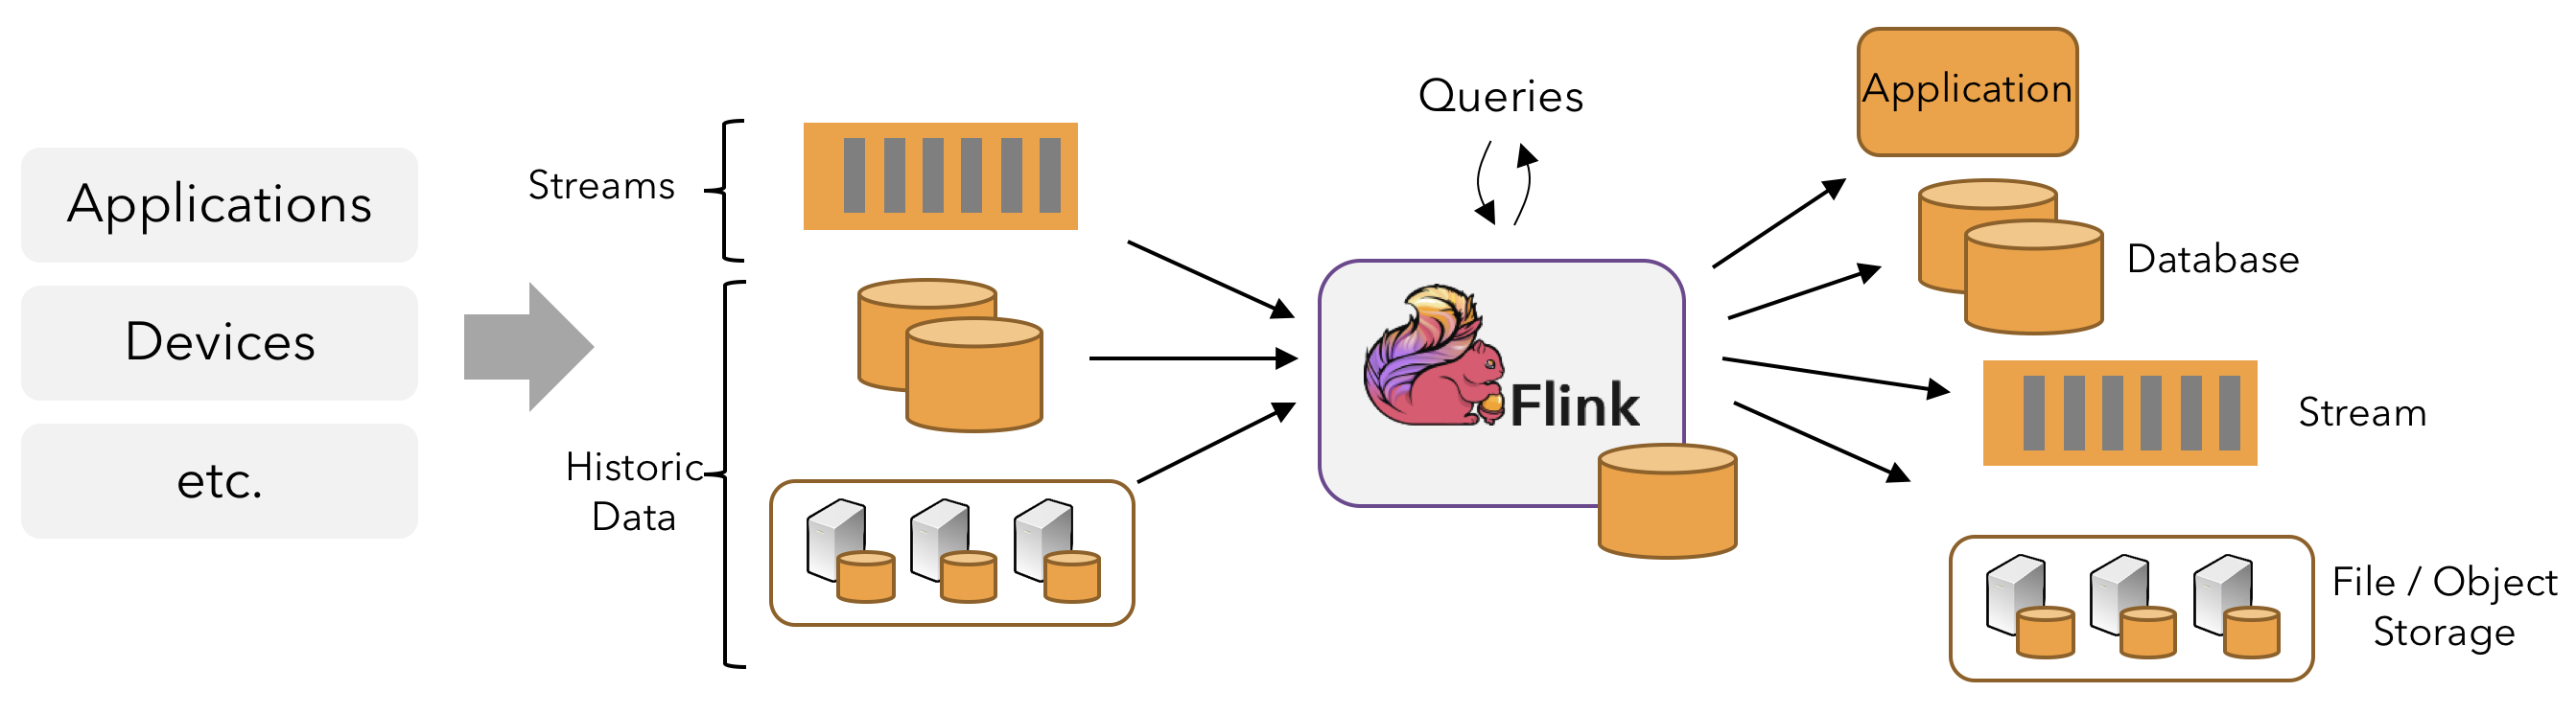
\includegraphics[width=\textwidth]{flink-app.png}
    \caption{Использование Apache Flink.}
    \label{fig:flink-app}
\end{figure}

Запросы задаются в виде вычислительного графа (пайплайна), который представляет собой ориентированный граф без циклов. Пример задания такого графа представлен на рисунке \ref{fig:prog-data}.

\begin{figure}
    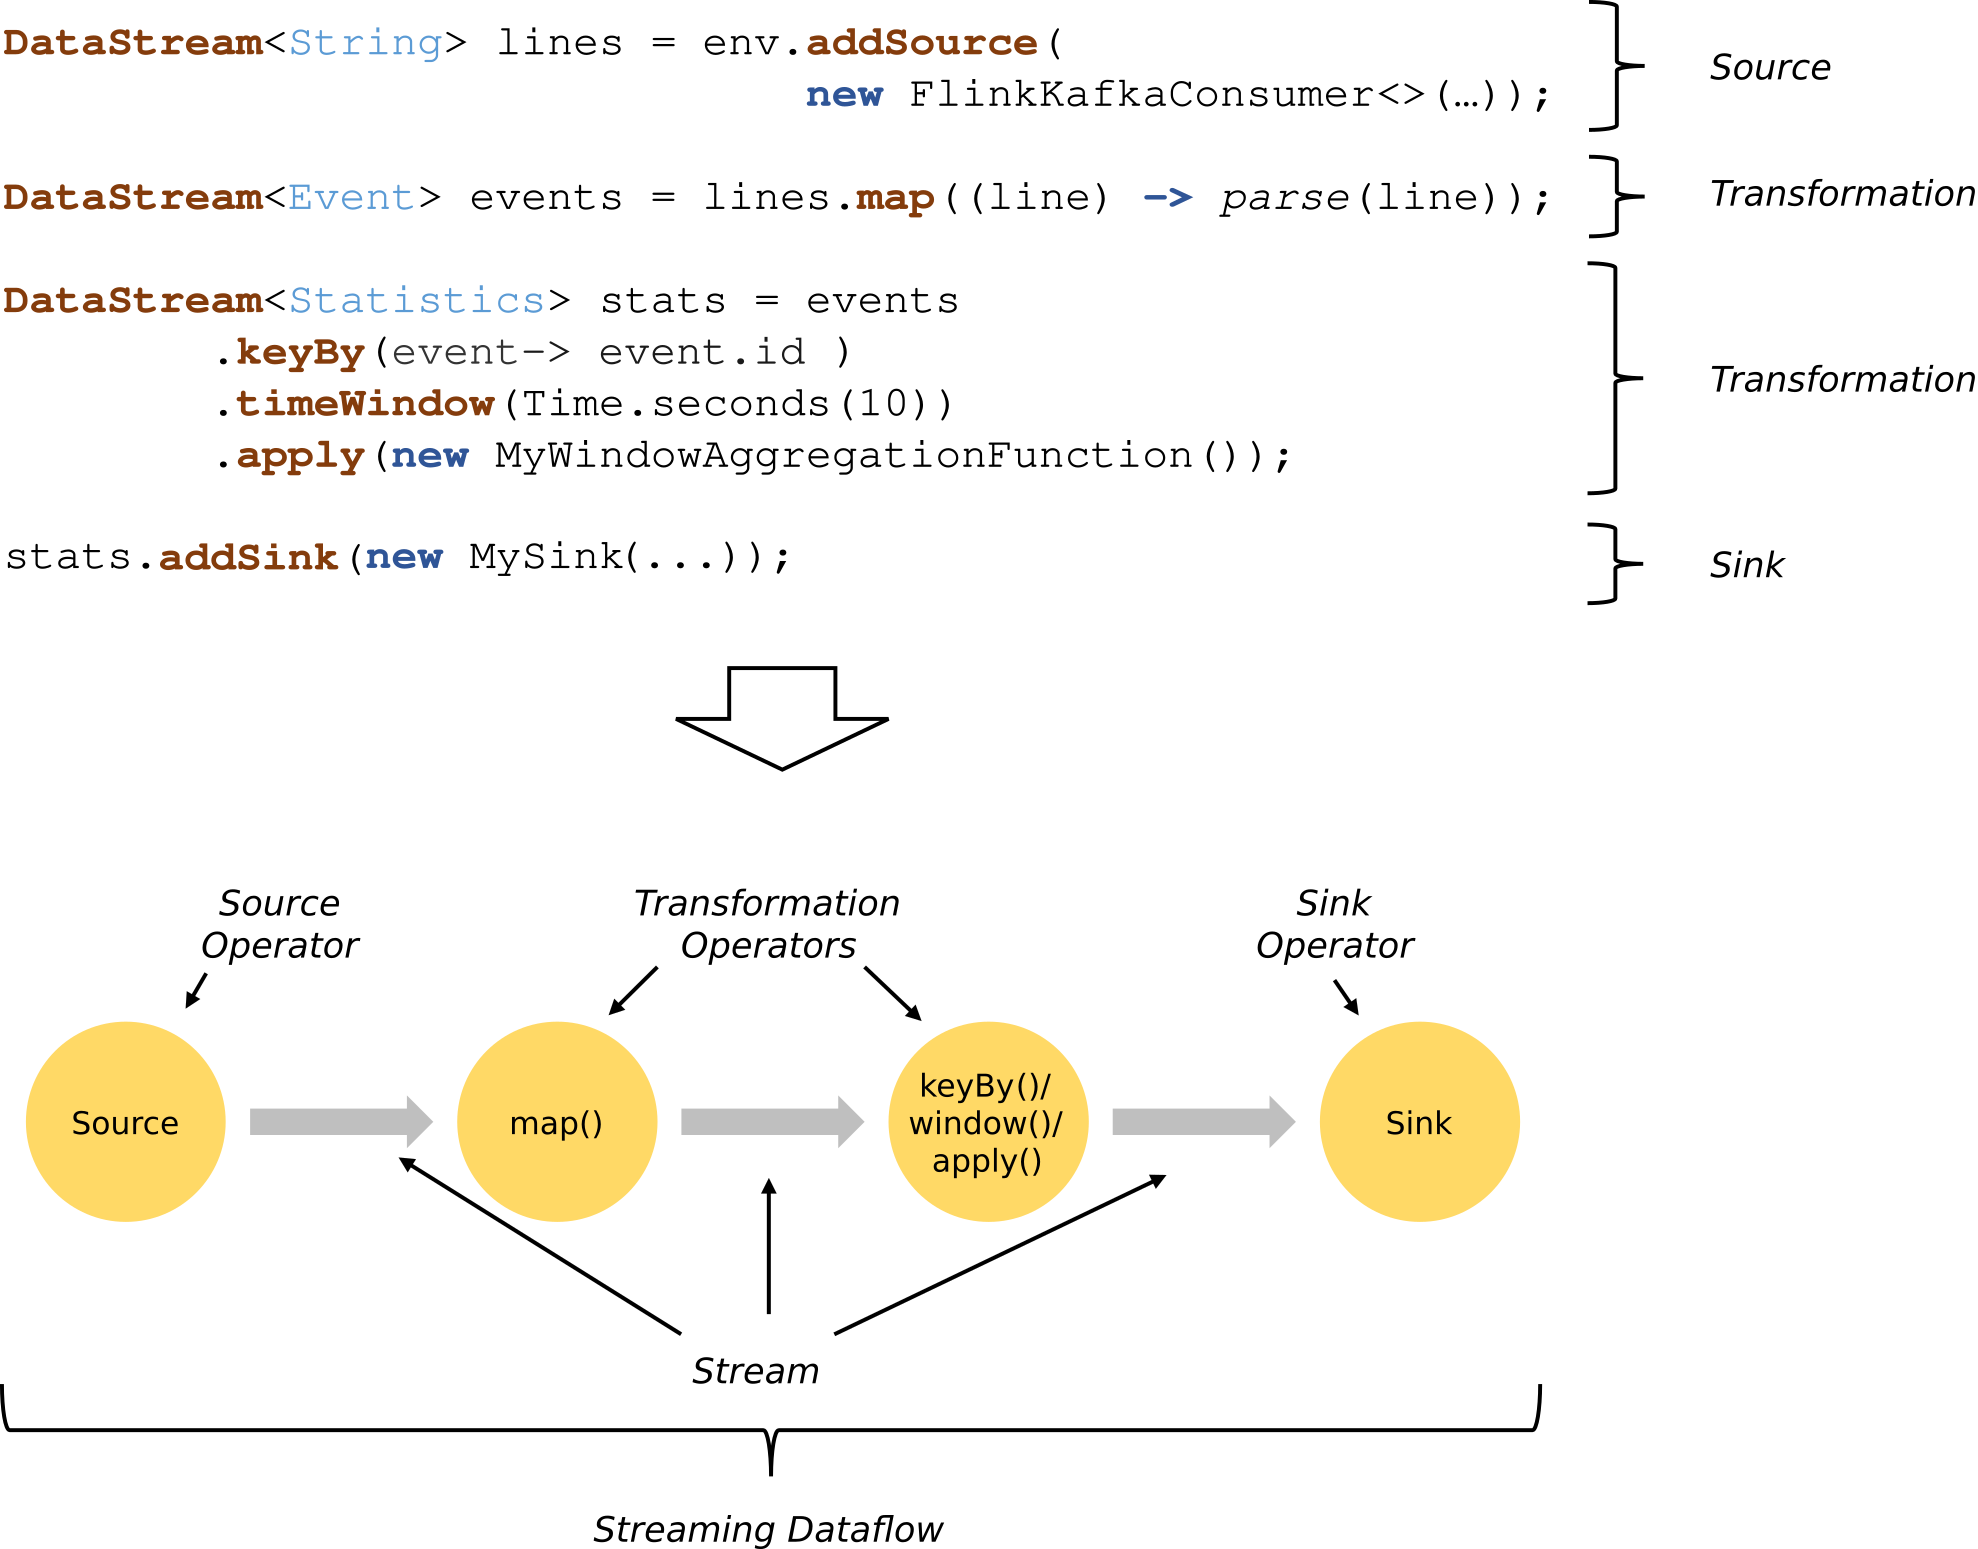
\includegraphics[width=\textwidth]{program_dataflow.png}
    \caption{Пример вычислительного графа для Apache Flink.}
    \label{fig:prog-data}
\end{figure}

Копии пайплайна распределяются между машинами для параллельной обработки данных.
Часть операций не содержат состояния и не требуют дополнительных усилий, чтобы быть запущенными в нескольких экземплярах и работать параллельно.
Некоторые операции же, такие как агрегация, требуют наличия изменяемого состояния и требуют специального перераспределения (решардирования) данных между их экземплярами (чтобы записи с одним и тем же ключём подсчитывались только на одной машине, например, и не было необходимости производить агрегацию по машинам). Пример показан на рисунке \ref{fig:par-data}.

\begin{figure}
    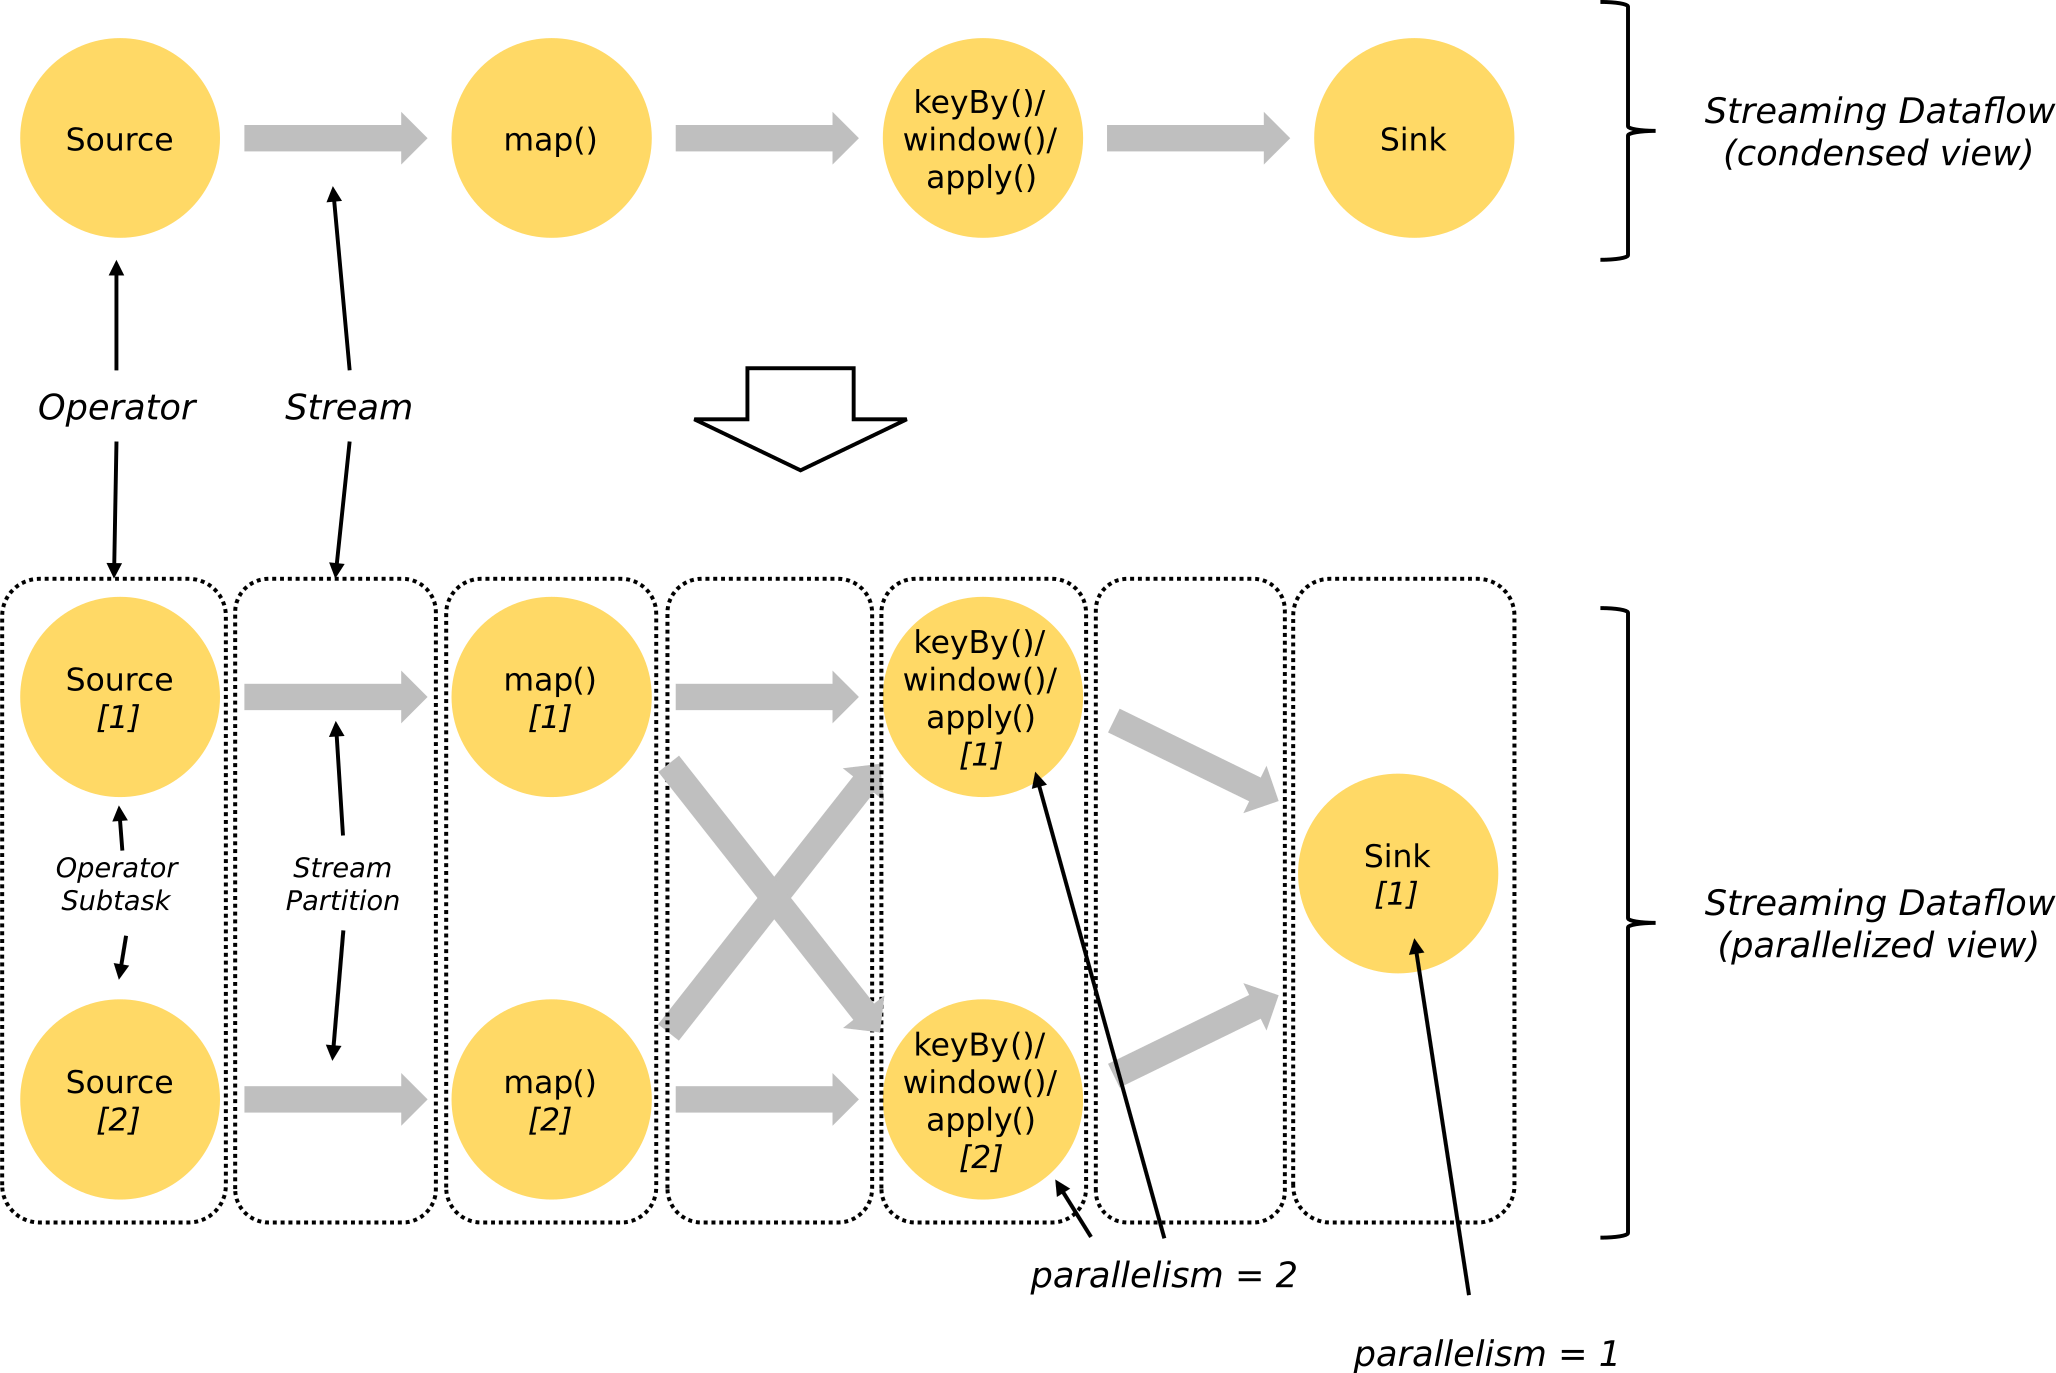
\includegraphics[width=\textwidth]{parallel_dataflow.png}
    \caption{Распределение данных между экземплярами операций одного и того же пайплайна, размещёнными на разных машиных. Операция \textit{map()} не имеет состояния, и её два экземпляра параллельно обрабатывают один и тот же поток данных, не влияя друг на друга. Операция \textit{apply()} же имеет изменяемое состояние, поэтому необходимо производить перераспределение данных (решардирование) между её экземплярами с помощью \textit{keyBy()}.}
    \label{fig:par-data}
\end{figure}

В данной работе предлагается новый способ задания вычислительных графов для распределённых потоковых систем, который позволяет упростить программирование комплексных пайплайнов и производить их автоматическую оптимизацию.

Все материалы работы можно найти в \href{https://github.com/winter-yuki/calco}{GitHub репозитории проекта}.
